\documentclass[crop,border={0pt 20pt 5pt 20pt}]{standalone}
\usepackage{tikz,fontspec,color}
\usetikzlibrary{hobby}   

\setmainfont{TeXGyreTermes}[
    Path = ../fonts/,
    UprightFont = *-Regular,
    BoldFont = *-Bold,
    ItalicFont = *-Italic,
    BoldItalicFont = *-BoldItalic]

\definecolor{color0}{HTML}{000000}
\definecolor{color1}{HTML}{00ACC1}
\definecolor{color2}{HTML}{000000}
\definecolor{color3}{HTML}{E53935}
\definecolor{color4}{HTML}{00ACC1}

\usepackage{pst-node,pst-plot}
\pstVerb{realtime srand}
\psset{plotpoints=30}
\def\points{}

\tikzstyle{conn} = [line width=.2mm]
\tikzstyle{circ} = [start angle=0, end angle=360]
\tikzstyle{elli} = [conn, closed=true, smooth]
\tikzstyle{lbls} = [text width=3cm, color0]

\begin{document}
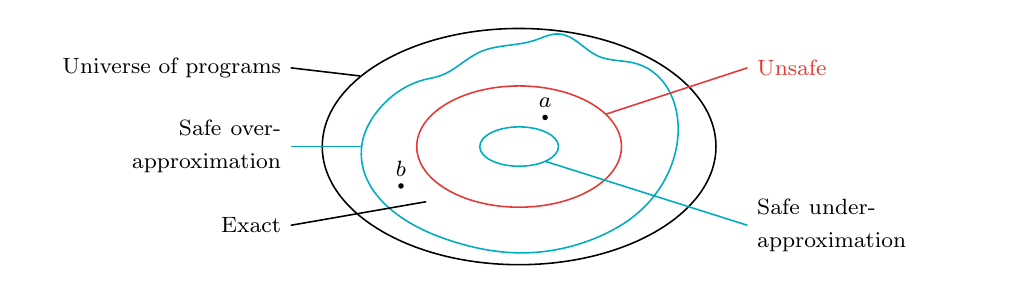
\begin{tikzpicture}
%\draw[gray!20!white,step=.5] (-6,-2) grid (6,2);
\draw[elli,color0] (2.5,0)  arc [circ, x radius=2.50, y radius=1.50] node [pos=.40,xshift=.3mm] (C0) {};
\draw[elli,color3] (1.3,0)  arc [circ, x radius=1.30, y radius=0.77] node [pos=.08,xshift=-2.6mm] (C3) {};
\draw[elli,color4] (0.5,0)  arc [circ, x radius=0.50, y radius=0.25] node [pos=.90,xshift=-3mm] (C4) {};
\coordinate (C1) at (-2.10, .0);
\coordinate (C2) at (-1.28,-.7);    
\fill ( .33,.37) circle (1pt) node[anchor=south] at ( .33,.37) {\footnotesize{$a$}};
\fill (-1.5,-.5) circle (1pt) node[anchor=south] at (-1.5,-.5) {\footnotesize{$b$}};

\path[elli,draw=color1,use Hobby shortcut]
   (-2.0, 0.00)
.. (-1.0,-1.15)   
.. ( 0.0,-1.35)   
.. ( 1.0,-1.15)
.. ( 1.5,-0.85)
.. ( 2.0, 0.00) 
.. ( 1.5, 1.05)
.. ( 1.0, 1.15)
.. ( 0.5, 1.43)
.. ( 0.2, 1.35)
.. (-0.5, 1.20)
.. (-1.0, 0.90)
.. (-1.2, 0.85)
.. (-1.8, 0.45); 

\begin{pspicture}(-.1,.25)(0, 0)
\psset{linecolor=color2,linewidth=.2mm}
\curvepnodes{0}{360}{Rand .5 add t PtoC}{X}
\multido{\i=0+1}{\Xnodecount}{\xdef\points{\points (X\i)}}
\expandafter\psccurve\points
\end{pspicture}

\coordinate [label={[color0]left:\footnotesize{Universe of programs}}]
(L0) at (-3, 1);
\coordinate [label={[lbls,color0, align=right]left:\footnotesize{Safe over-approximation}}] 	
(L1) at (-3, 0);
\coordinate [label={[color2]left:\footnotesize{Exact}}]
(L2) at (-3, -1);
\coordinate [label={[lbls,color3]right:\footnotesize{Unsafe}}]
(L3) at (2.8, 1);
\coordinate [label={[lbls,color0]right:\footnotesize{Safe under-approximation}}] 					
(L4) at (2.8, -1);

\draw[conn,color0] (L0) -- (C0);
\draw[conn,color1] (L1) -- (C1);
\draw[conn,color2] (L2) -- (C2);
\draw[conn,color3] (L3) -- (C3);
\draw[conn,color4] (L4) -- (C4);  

\end{tikzpicture}
\end{document}